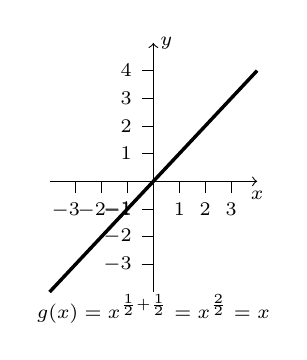
\begin{tikzpicture}
  \begin{axis}[
    width=120pt,
    height=135pt,
    xmin=-4, xmax=4,
    ymin=-4, ymax=5,
    axis lines=middle,
    x axis line style={->},
    y axis line style={->},
    xtick={-3,-2,-1,1,2,3},
    ytick={-1,-2,-3,1,2,3,4},
    xticklabels={{\scriptsize $-3 \hspace{7pt}$},{\scriptsize $-2 \hspace{7pt}$},{\scriptsize $-1 \hspace{7pt}$},{\scriptsize $1$},{\scriptsize $2$},{\scriptsize $3$}},
    yticklabels={{\scriptsize $-1$},{\scriptsize $-2$},{\scriptsize $-3$},{\scriptsize $1$},{\scriptsize $2$},{\scriptsize $3$},{\scriptsize $4$}},
    tick style={black},
    tick align=outside,
    clip=false
  ]
    \addplot[line width=1.25pt] coordinates {(-4,-4) (4,4)};
    \node at (axis cs:4,-0.5) {\scriptsize $x$};
    \node at (axis cs:0.5,5) {\scriptsize $y$};
  \end{axis}
  \path (current axis.south) ++(0,-6pt) node {\scriptsize $g(x) =  x^{\frac{1}{2} + \frac{1}{2}} = x^{\frac{2}{2}} = x$ };
\end{tikzpicture}